\documentclass[11pt]{article}

\usepackage{fullpage}
\usepackage{enumerate}
\usepackage{natbib}
\usepackage{graphicx}
\usepackage{hyperref}
\usepackage{ifthen}
\usepackage[all]{hypcap}
\newcommand{\logfig}[2]{
See figure~\ref{fig:#1}.
\begin{figure}[!ht] 
\includegraphics[width=0.8\textwidth]{#1} 
\caption{#2} 
\label{fig:#1} 
\end{figure}
}

\bibliographystyle{aa_arxiv}

\def\aj{AJ}%
          % Astronomical Journal
\def\araa{ARA\&A}%
          % Annual Review of Astron and Astrophys
\def\apj{ApJ}%
          % Astrophysical Journal
\def\apjl{ApJ}%
          % Astrophysical Journal, Letters
\def\apjs{ApJS}%
          % Astrophysical Journal, Supplement
\def\aap{A\&A}%
          % Astronomy and Astrophysics
\def\aapr{A\&A~Rev.}%
          % Astronomy and Astrophysics Reviews
\def\aaps{A\&AS}%
          % Astronomy and Astrophysics, Supplement
\def\jcap{JCAP}%
          %Journal of Cosmology and Astroparticle Physics
\def\mnras{MNRAS}%
          % Monthly Notices of the RAS
\def\nat{Nature}%
          % Nature
\def\pasj{PASJ}%
          % Publications of the Astronomical Society of Japan
\def\pasp{PASP}%
          % Publications of the ASP
\def\physrep{Phys.~Rep.}%
          % Physics Reports
\def\prd{Phys.~Rev.~D}
          % Physical Review D
\let\apjlett=\apjl


\title{Analysis Document: Weak Lensing Calibration with N-body Simulations}
\date{Started ~Feb 2013}
\author{Douglas Applegate}


\begin{document}

\maketitle

\tableofcontents

%%%%%%%%%%%%%%%%%%%%%%%%%%%%%%%%%%%%%%%%%%%%%%%%%%%%%%%%%%%%%

\section{Project Description}

The goal of this project is to measure and improve the systematic uncertainty from mass-profile modeling in weak lensing. In the Weighing the Giants analysis, we assumed an NFW density profile. Does that bias the mean mass of the sample? How well can we constrain that bias? Starting at that point, I am to answer some of the following questions:

\begin{itemize}
\item What is the bias when you fit an NFW halo? What is the optimal radial range to fit, in terms of bias, systematic uncertainty and statistical uncertainty?
\item Is the NFW profile the best description? Do other profiles work better? Are there other ways to measure masses (eg Mass Aperture) that are better?
\item How does this evolve with cluster mass, and with redshift? Are there other predictors?
\item How do we best handle the mass-concentration relation?
\item How do we best handle the prior on cluster mass?
\item Are there differences in predictions from different simulations, and from different ways to simulate lensing?
\end{itemize}

The simulations may also give insights into more advanced topics, such as 
\begin{itemize}
\item What can simulations tell us about applying contamination corrections?
\item Can we measure cluster concentrations?
\item Can we measure cluster ellipticities, and over what radial range?
\item If designing a survey from scratch, how should we do it?
\end{itemize}

There are currently three analysis efforts that these results feed into. The first is the Stanford Weighing the Giants work, with Steve, Adam, and Anja, working with wide field, ground-based observations from Subaru. Then there is the SPT efforts at low and high redshifts, with Tim and Joerg. The high-z work uses HST observations, whereas the low-z work uses Megacam @ Magellan. Finally, this work also feeds into the LSST effort.


%%%%%%%%%%%%%%%%%%%%%%%%%%%%%%%%%%%%%%%%%%%%%%%%%%%%%%%%%%%%%%%%%%%%%%%%%%%%%%%%%%%%%%%%%%%%%%%%%%%%%%%%%%%%%%%%%%%%%%%%%%%%%%%%%%%%%%%%%%%%%%%%%%%%%%%%%%%%%%%%%%%%%%%%%%%%%%%%%%%%%%%%%%%%%%%%%%%%%%%%%%%%
%%%%%%%%%%%%%%%%%%%%%%%%%%%%%%%%%%%%%%%%%%%%%%%%%%%%%%%%%%%%%%%%%%%%%%%%%%%%%%%%%%%%%%%%%%%%%%%%%%%%%%%%%%%%%%%%%%%%%%%%%%%%%%%%%%%%%%%%%%%%%%%%%%%%%%%%%%%%%%%%%%%%%%%%%%%%%%%%%%%%%%%%%%%%%%%%%%%%%%%%%%%%
%%%%%%%%%%%%%%%%%%%%%%%%%%%%%%%%%%%%%%%%%%%%%%%%%%%%%%%%%%%%%%%%%%%%%%%%%%%%%%%%%%%%%%%%%%%%%%%%%%%%%%%%%%%%%%%%%%%%%%%%%%%%%%%%%%%%%%%%%%%%%%%%%%%%%%%%%%%%%%%%%%%%%%%%%%%%%%%%%%%%%%%%%%%%%%%%%%%%%%%%%%%%
\clearpage \newpage


\section{Log}

\paragraph{15 July 2013}
Lots of development work during the March period that was undocumented. 
Basically, got running on Becker's simulations. 
Oddly, though, I couldn't reproduce his results. 
Not sure why, but it may be because I am only looking at the most massive halos while he was fitting biases to all halos.
While there are many things that I can do to try to recover Matt's results, I don't know if I can.
First step is to go back to my results, and just figure out what is going on.


\paragraph{01 Jan 2013}
Start of this work package. 
First step is to clean up old code that I've been using in bonnpipeline and get it running with Will's simulated catalogs.

\paragraph{06 Aug 2013}
I've recieved from Jiayi in Munich a distribution of SZ - halo center offsets from a new set of hydro sims they've done. I'm going to explore the offset distributions and effects on an NFW halo in an ipython notebook called: simulated\_offsets.ipynb .

\paragraph{19 Feb 2014}
After a long gap in this notebook, I'm back to updating it and tracking my research investigations. Since I've last updated, I've added two new simulation sets, the BCC and the MXXL. I've implemented a uniform analysis, and have begun exploring different radial ranges, as well as differences between the two simulations. I've updated all sections of the notebook to try to capture these pieces.

\paragraph{21 Feb 2014}
Setting up simulations for two different experiments: understanding the noise and bias tradeoffs for the HST simulations, and understanding the effect of decreased sampling density and increased shape noise. Added configuration files, and utilities to generate configuration files. Modifications to nfwfit and associated software to deal with subsampling, shifting to different redshifts, and adding shape noise.

\paragraph{24 Feb 2014}
Looking at results from changing noise \& sampling density in MXXL and BCC. See section~\ref{sec:noisebias}.
Also looking at predictions for noise and bias for proposed HST snapshot programs. See section~\ref{sec:hstproposal}.

\paragraph{25 Feb 2014}
Looked at the results for the HST mock-ups. There was a bug, in that I forgot to change the area accepted when I pretend clusters are at different redshifts. Rerunning that.

\paragraph{26 Feb 2014}
While I'm rerunning the HST stuff, I wanted to look at the posterior of a few individual clusters. See section~\ref{sec:noisebias_posteriors}.

\paragraph{27 Feb 2014}
Starting to set up a few more explorations: binning \& cosmology-dependent mass-concentration relation.

\paragraph{28 Feb 2014}
Attempting to catch up on my notes from this last week. Need to add info on noise effects(sec~\ref{sec:noisebias}) and the hst proposal (sec~\ref{sec:hstproposal}).


%%%%%%%%%%%%%%%%%%%%%%%%%%%%%%%%%%%%%%%%%%%%%%%%%%%%%%%%%%%%%%%%%%%%%%%%%%%%%%%%%%%%%%%%%%%%%%%%%%%%%%%%%%%%%%%%%%%%%%%%%%%%%%%%%%%%%%%%%%%%%%%%%%%%%%%%%%%%%%%%%%%%%%%%%%%%%%%%%%%%%%%%%%%%%%%%%%%%%%%%%%%%
%%%%%%%%%%%%%%%%%%%%%%%%%%%%%%%%%%%%%%%%%%%%%%%%%%%%%%%%%%%%%%%%%%%%%%%%%%%%%%%%%%%%%%%%%%%%%%%%%%%%%%%%%%%%%%%%%%%%%%%%%%%%%%%%%%%%%%%%%%%%%%%%%%%%%%%%%%%%%%%%%%%%%%%%%%%%%%%%%%%%%%%%%%%%%%%%%%%%%%%%%%%%
%%%%%%%%%%%%%%%%%%%%%%%%%%%%%%%%%%%%%%%%%%%%%%%%%%%%%%%%%%%%%%%%%%%%%%%%%%%%%%%%%%%%%%%%%%%%%%%%%%%%%%%%%%%%%%%%%%%%%%%%%%%%%%%%%%%%%%%%%%%%%%%%%%%%%%%%%%%%%%%%%%%%%%%%%%%%%%%%%%%%%%%%%%%%%%%%%%%%%%%%%%%%
\clearpage \newpage


\section{Guide to Files \& Software}

TODO: Fill in guide to software



%%%%%%%%%%%%%%%%%%%%%%%%%%%%%%%%%%%%%%%%%%%%%%%%%%%%%%%%%%%%%%%%%%%%%%%%%%%%%%%%%%%%%%%%%%%%%%%%%%%%%%%%%%%%%%%%%%%%%%%%%%%%%%%%%%%%%%%%%%%%%%%%%%%%%%%%%%%%%%%%%%%%%%%%%%%%%%%%%%%%%%%%%%%%%%%%%%%%%%%%%%%%
%%%%%%%%%%%%%%%%%%%%%%%%%%%%%%%%%%%%%%%%%%%%%%%%%%%%%%%%%%%%%%%%%%%%%%%%%%%%%%%%%%%%%%%%%%%%%%%%%%%%%%%%%%%%%%%%%%%%%%%%%%%%%%%%%%%%%%%%%%%%%%%%%%%%%%%%%%%%%%%%%%%%%%%%%%%%%%%%%%%%%%%%%%%%%%%%%%%%%%%%%%%%
%%%%%%%%%%%%%%%%%%%%%%%%%%%%%%%%%%%%%%%%%%%%%%%%%%%%%%%%%%%%%%%%%%%%%%%%%%%%%%%%%%%%%%%%%%%%%%%%%%%%%%%%%%%%%%%%%%%%%%%%%%%%%%%%%%%%%%%%%%%%%%%%%%%%%%%%%%%%%%%%%%%%%%%%%%%%%%%%%%%%%%%%%%%%%%%%%%%%%%%%%%%%
\clearpage \newpage


\section{Available Simulations}

I have access to 3 sets of simulations:

\paragraph{BK11} : Cut-outs around massive halos at redshifts z=0.25 and z=0.5, used in Becker \& Kravtsov 2011. Particles are extracted in a 20x20x400 comoving Mpc/h box around each cluster and are projected to form a 2-D mass map. From that, a shear signal is calculated, assuming sources are at z=1

\paragraph{BCC} : A simulation of a large sky-area survey covering a continuous patch of sky. Three boxes of decreasing resolution are appended and are used to form a past light cone of the visible universe. The simulation ray-traces shear from each galaxy in the simulation to the observer at z=0. I have extracted galaxies centered around the lensed central position of each massive halo in the simulation. From Wechsler, Becker, and Buscha, priv comm.

\paragraph{MXXL}: A large box where snapshots at particular redshifts are written to disk. I currently have only the z=1 snapshot. Sources are assumed to be at infinite distance (not infinite redshift). Shear is calculated by projecting masses to a plane in a box (of unknown size) around each massive cluster. I have 3 projections for each cluster.


%%%%%%%%%%%%%%%%%%%%%%%%%%%%%%%%%%%%%%%%%%%%%%%%%%%%%%%%%%%%%%%%%%%%%%%%%%%%%%%%%%%%%%%%%%%%%%%%%%%%%%%%%%%%%%%%%%%%%%%%%%%%%%%%%%%%%%%%%%%%%%%%%%%%%%%%%%%%%%%%%%%%%%%%%%%%%%%%%%%%%%%%%%%%%%%%%%%%%%%%%%%%
%%%%%%%%%%%%%%%%%%%%%%%%%%%%%%%%%%%%%%%%%%%%%%%%%%%%%%%%%%%%%%%%%%%%%%%%%%%%%%%%%%%%%%%%%%%%%%%%%%%%%%%%%%%%%%%%%%%%%%%%%%%%%%%%%%%%%%%%%%%%%%%%%%%%%%%%%%%%%%%%%%%%%%%%%%%%%%%%%%%%%%%%%%%%%%%%%%%%%%%%%%%%
%%%%%%%%%%%%%%%%%%%%%%%%%%%%%%%%%%%%%%%%%%%%%%%%%%%%%%%%%%%%%%%%%%%%%%%%%%%%%%%%%%%%%%%%%%%%%%%%%%%%%%%%%%%%%%%%%%%%%%%%%%%%%%%%%%%%%%%%%%%%%%%%%%%%%%%%%%%%%%%%%%%%%%%%%%%%%%%%%%%%%%%%%%%%%%%%%%%%%%%%%%%%
\clearpage \newpage


\section{Are the simulations consistent?}

In the most basic test, do I recover the same bias as a function of mass from each simulation? There are a few reasons why I might not. 

\begin{itemize}
\item Each simulation probes a different redshift range, so I should be able to probe redshift evolution. Thankfully, the BCC bridges between the MXXL and BK11, while I will also hopefully receive additional snapshots from the MXXL. 
\item Each simulation uses a slightly different cosmology. That may mean that the mass-concentration relations are different, which may again lead to different biases. 
\item Each simulation is at different resolutions, so there could be resolution issues, especially near the cluster centers. 
\item The BCC ray traces over a past light cone, whereas BK11 and the MXXL ignore LSS evolution and don't ray trace
\item The density of points where the shear field is measured is different. Bahe+2012 shows that lower density surveys / noisier surveys average over / miss some substructure, leading to different bias results.
\item There may be a bug in how I'm reading in one of the simulations. This was previously a problem with the BK11 simulations, where I first missed factors of h, and then there was ambiguity about at what redshift the lensing signal was calculated for.
\end{itemize}

\subsection{Basic Analysis Approach}

TODO: Fill in details here on how exactly I do my fits.

The fit is encoded in nfwfit.py. 


\subsection{Comparing Mass Bias vs Radial Range \& M-C Relation}
\label{sec:consistant_bias_mcrelation}

I've run mass fits with three mass-concentration relations: c=4, the Duffy08 relation, and allowing c to be fit freely.

I've run fits for 15 different radial ranges: 3 Inner radii {0.25, 0.5, 0.75 Mpc}, and 6 outer radii {0.5, 0.75, 1.0, 1.5, 2.5, 3.0}. The radial ranges are encoded as follows:

\begin{itemize}
\item 'r1' : '0.25 - 0.5 Mpc',
\item 'r2' : '0.25 - 1.5 Mpc',
\item 'r3' : '0.25 - 2.5 Mpc',
\item 'r4' : '0.25 - 3.0 Mpc',
\item 'r5' : '0.50 - 1.5 Mpc',
\item 'r6' : '0.50 - 2.5 Mpc',
\item 'r7' : '0.50 - 3.0 Mpc',
\item 'r8' : '0.75 - 1.5 Mpc',
\item 'r9' : '0.75 - 2.5 Mpc',
\item 'r10' :'0.75 - 3.0 Mpc',
\item 'r11' :'0.25 - 0.75 Mpc',
\item 'r12' :'0.25 - 1.0 Mpc',
\item 'r13' :'0.50 - 0.75 Mpc',
\item 'r14' :'0.50 - 1.0 Mpc',
\item 'r15' :'0.75 - 1.0 Mpc'
\end{itemize}


When I assume either c=4 or Duffy08, I see that the simulations produce different results. The slopes of bias vs mass change, as well as the absolute normalizations. The three simulations appear to respond differently as well. See figure~\ref{fig:comparing_r7_bias}. The curves seem to shift some between simulations. But since I am refitting the same halos, I would expect that the shifts in each simulation are real. Only when I go to cfree are the BCC and MXXL seemingly consistent. BK11 is hanging out by itself for some reason, which I don't understand.

\begin{figure} \centering[!ht]
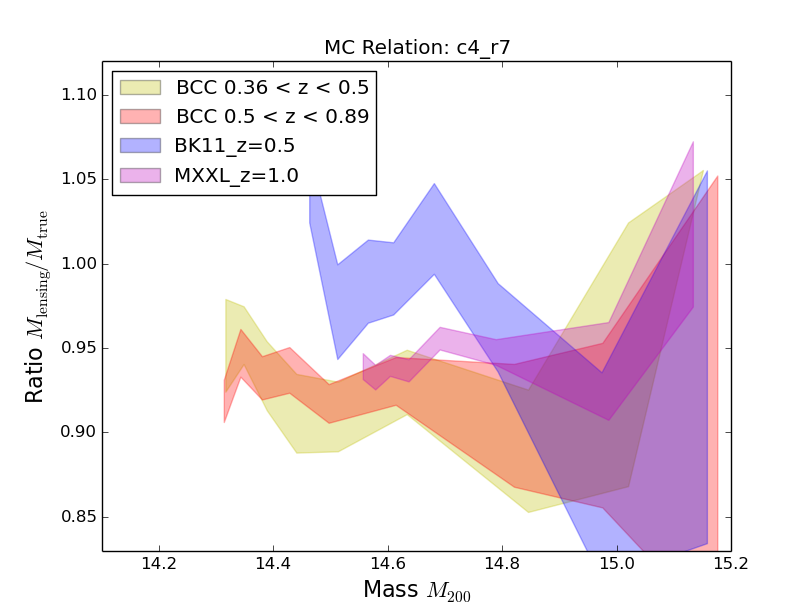
\includegraphics[width=0.3\textwidth]{figures/c4_r7}
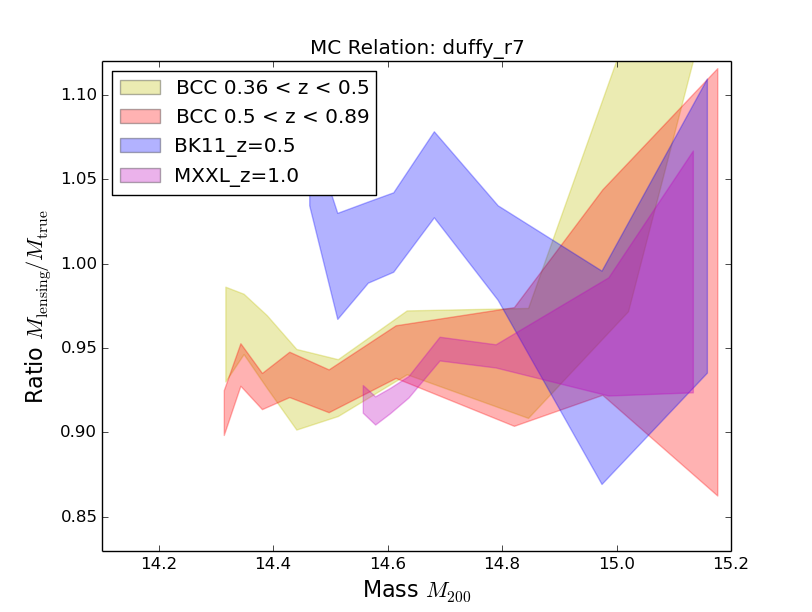
\includegraphics[width=0.3\textwidth]{figures/duffy_r7}
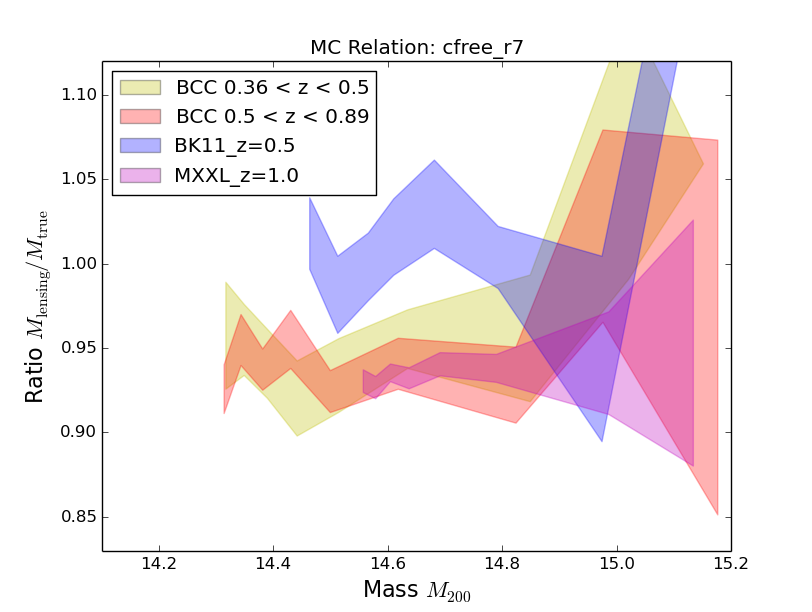
\includegraphics[width=0.3\textwidth]{figures/cfree_r7}
\caption{Plot of bias versus mass. Left: Assuming c=4, Center: Assuming Duffy08, and Right: C is a free parameter. The fit range is 0.5 - 3.0 Mpc. The width of each colored band represents the $1\sigma$ uncertainty in the median bias for each mass bin. Bins are adaptively created to balance signal-to-noise with exploring the mass range. Made with compareDiffSims.py}
\label{fig:comparing_r7_bias}
\end{figure}

The agreement between BCC and MXXL seems to be fit range dependent. The above fits covered a range of 0.5 - 3.0 Mpc. If we only look at the outer region for cfree, the fits are again good.

\logfig{figures/cfree_r10}{Same as fig~\ref{fig:comparing_r7_bias}, except now only for cfree and 0.75-3Mpc.}

However, if we look at the innermost fit region, 0.25-0.5 mpc, we can see that the two simulations are drastically different. BCC and BK11 show diving calibrations at the high mass end (0.2 for $10^{15}$ halos!?), but MXXL holds relatively steady up to the highest masses. 

\logfig{figures/cfree_r1}{Same as fig~\ref{fig:figures/cfree_r10}, except for on a radically different scale.}

Could this be a resolution effect? Or maybe how the shear signal is calculated, since we are getting close to the critical curves, though I would think if that was the case BK11 and MXXL would be more consistent. We also should only be seeing shears of $g\approx0.3$ at 250kpc for z=1 and $10^{15}$ solar masses.


\subsection{Role of Mass-Concentration Relation}

I think that the behavior of the fits against the different mass-concentration relations vs cfree suggests that the simulations have intrinsically different m-c relations. This is supported by the work of \citet{ludlow_mc}, which shows that even for $M_{200} = 10^{14}$ clusters, the mean concentration can vary by 20\% over the WMAP1-7 and Planck cosmologies. 

This to me suggests a 2-pronged strategy. When we don't care about cosmology, for example, just talking about masses, then we can fix a mass-concentration relation (appropriate for that cosmology). However, for purposes of cosmological fits, we need to vary the m-c relation systematically over all clusters inline with the fit. That way we don't get hit by some ``systematic uncertainty'' by assuming an M-C relation, and we capture the covariance with cosmology.


\subsection{Next Steps}

\begin{itemize}
\item I want to stack cluster shear profiles (grouping by mass, redshift, and concentration), and see if I can visually see differences at low redshifts. Maybe I should stack residuals? That might confirm my suspicion that there is some sort of different treatment or resolution effect afflicting cluster cores in BCC and BK11.
\item I should implement the Ludlow prescription for cosmology-dependent m-c relations. I should then check to see if I get a consistant bias across all three simulations/cosmologies. That would confirm my suspicion about how to treat the m-c relation, while being robust to non-consenus parameter values.
\end{itemize}


%%%%%%%%%%%%%%%%%%%%%%%%%%%%%%%%%%%%%%%%%%%%%%%%%%%%%%%%%%%%%%%%%%%%%%%%%%%%%%%%%%%%%%%%%%%%%%%%%%%%%%%%%%%%%%%%%%%%%%%%%%%%%%%%%%%%%%%%%%%%%%%%%%%%%%%%%%%%%%%%%%%%%%%%%%%%%%%%%%%%%%%%%%%%%%%%%%%%%%%%%%%%
%%%%%%%%%%%%%%%%%%%%%%%%%%%%%%%%%%%%%%%%%%%%%%%%%%%%%%%%%%%%%%%%%%%%%%%%%%%%%%%%%%%%%%%%%%%%%%%%%%%%%%%%%%%%%%%%%%%%%%%%%%%%%%%%%%%%%%%%%%%%%%%%%%%%%%%%%%%%%%%%%%%%%%%%%%%%%%%%%%%%%%%%%%%%%%%%%%%%%%%%%%%%
%%%%%%%%%%%%%%%%%%%%%%%%%%%%%%%%%%%%%%%%%%%%%%%%%%%%%%%%%%%%%%%%%%%%%%%%%%%%%%%%%%%%%%%%%%%%%%%%%%%%%%%%%%%%%%%%%%%%%%%%%%%%%%%%%%%%%%%%%%%%%%%%%%%%%%%%%%%%%%%%%%%%%%%%%%%%%%%%%%%%%%%%%%%%%%%%%%%%%%%%%%%%
\clearpage \newpage



\section{Optimal Radial Ranges for NFW Profiles}

Question: What is the best radial range to use when fitting an NFW profile? I need to provide answers in two different regiemes, which in the end may end up overlapping. The first is the SPT regime, where the limited field of view on Hubble restricts how far out we can probe. The second regime is ground-based wide-field data from Subaru or LSST, where we can go out as far as we want.

I ran 15 different fit ranges (see~\ref{sec:consistant_bias_mcrelation}) for all 3 simulations. Right now I am biased towards MXXL, so I will only show results for that at the moment.

\logfig{figures/cfree}{Plotting mass bias from lensing versus cluster mass, using the MXXL simulation and no m-c relation, for different radial ranges. Line styles denote different inner fit boundaries, while color denotes different outer fit boundaries. Color are grouped, suggesting that the outer fit boundary is more important than the inner fit boundary. Produced with compareSims.py}

Outer fit range seems to matter much more than inner fit range. You might expect that the behavior changes as the fit includes or excludes r200. R200 is at ~1.1Mpc for $10^{14.5}$ clusters, whereas it is closer to 1.4Mpc for $10^{15}$ clusters. So for example, fitting out to 1Mpc is inside R200 for all clusters, and that bias seems to stay pretty level for all masses (the last bin is noisy). The pink line, fitting to 1.5mpc, is somewhat outside R200 for the lighter clusters, and just barely outside for the most massive -- that line shows larger cluster masses at higher true masses. If for some reason fitting m\&c biases masses up, then the pink line could be converging to the ``right'' answer at higher masses. Similar story for 2.5 and 3 Mpc, where masses are notably underestimated at low masses, and the trend heads to less bias at higher masses. I'm not sure how to explain the green lines, fitting to only 750kpc. 


\textbf{Could I fit perfect NFW halos and add noise? That way I could see the effects of noise bias on a two parameter fit?}


\logfig{figures/cfree_scatter}{Plotting intrinsic scatter versus mass for different radial ranges, using the MXXL simulation and no m-c relation. Same coloring and line scheme as fig.~\ref{fig:figures/cfree}. Scatter increases as I limit the outer radius used in the fit.}

The story with the scatter is much clearer. As I move the outer radial range to small values, the amount of scatter picks up. As soon as I move inside R200, the scatter blows up. Why is this? Smaller area, so subject to more LSS noise? More substructure in clusters?

\subsection{Next Steps}

For the HST proposal (due to STSCI in April, but need it for proposal writing by 25 Feb 2014), I need to add shape noise, use a lower sampling density, and apply HST masks associated with our mosaicing programs. That way I can directly measure the expected scatter for different choices, which will affect how powerful the HST program will be. 

There are some more general steps that I would like to do as well:
\begin{itemize}
\item Noise. I want to understand how the 2-parameter fit responds to noise. I could create perfect NFW halos and add shape noise to see how the best fit value changes. I also want to explore the 2D posterior surface for some of the clusters in MXXL, both relaxed and unrelaxed. Related, how does the posterior perform when I marginalize over it instead of using a point estimator?
\item We may in the end use a 1-parameter fit, but since the M-C relation is cosmology dependent, I need to implement a cosmology dependent relation. How does that perform?
\end{itemize}



%%%%%%%%%%%%%%%%%%%%%%%%%%%%%%%%%%%%%%%%%%%%%%%%%%%%%%%%%%%%%%%%%%%%%%%%%%%%%%%%%%%%%%%%%%%%%%%%%%%%%%%%%%%%%%%%%%%%%%%%%%%%%%%%%%%%%%%%%%%%%%%%%%%%%%%%%%%%%%%%%%%%%%%%%%%%%%%%%%%%%%%%%%%%%%%%%%%%%%%%%%%%
%%%%%%%%%%%%%%%%%%%%%%%%%%%%%%%%%%%%%%%%%%%%%%%%%%%%%%%%%%%%%%%%%%%%%%%%%%%%%%%%%%%%%%%%%%%%%%%%%%%%%%%%%%%%%%%%%%%%%%%%%%%%%%%%%%%%%%%%%%%%%%%%%%%%%%%%%%%%%%%%%%%%%%%%%%%%%%%%%%%%%%%%%%%%%%%%%%%%%%%%%%%%
%%%%%%%%%%%%%%%%%%%%%%%%%%%%%%%%%%%%%%%%%%%%%%%%%%%%%%%%%%%%%%%%%%%%%%%%%%%%%%%%%%%%%%%%%%%%%%%%%%%%%%%%%%%%%%%%%%%%%%%%%%%%%%%%%%%%%%%%%%%%%%%%%%%%%%%%%%%%%%%%%%%%%%%%%%%%%%%%%%%%%%%%%%%%%%%%%%%%%%%%%%%%
\clearpage \newpage

\section{What are the effects of noise and sampling density on bias \& scatter?}
\label{sec:noisebias}

\subsection{Motivation}
I'm doing nonlinear fits to noisy data, and taking point estimates of the posterior. We generally expect that doing that will produce biased results. It may also explain the differences between BCC, MXXL and BK11 simulations. While all three simulations are noise-free, shear fields are sampled at different densities, which may have an effect.

\subsection{Set up}

I have submitted runs on the MXXL and BCC with different densities. All of the following are galaxies(samples) per square arcminute.
\begin{itemize}
\item 0: Default density
\item 1: 100 (MXXL only)
\item 2: 20 (MXXL only)
\item 3: 20
\item 4: 7
\item 5: 4  (MXXL only)
\item 6: 1  (MXXL only)
\end{itemize}

I have used four different noise levels.
\begin{itemize}
\item 0: No noise
\item 1: 0.16 shape noise on tangential shear
\item 2: 0.33
\item 3: 0.5
\end{itemize}

I ran with c4 and cfree MC relations using the standard nfwfit.py software. Comparisons were made using the script compareSampling.py, and with the logfile compareSampling.log.


%%%%%%%%

\subsection{Does MXXL and BCC agree when using the same sampling density?}

We already know that the two simulations don't agree if c=4, so I will skip that.


\begin{figure} \centering
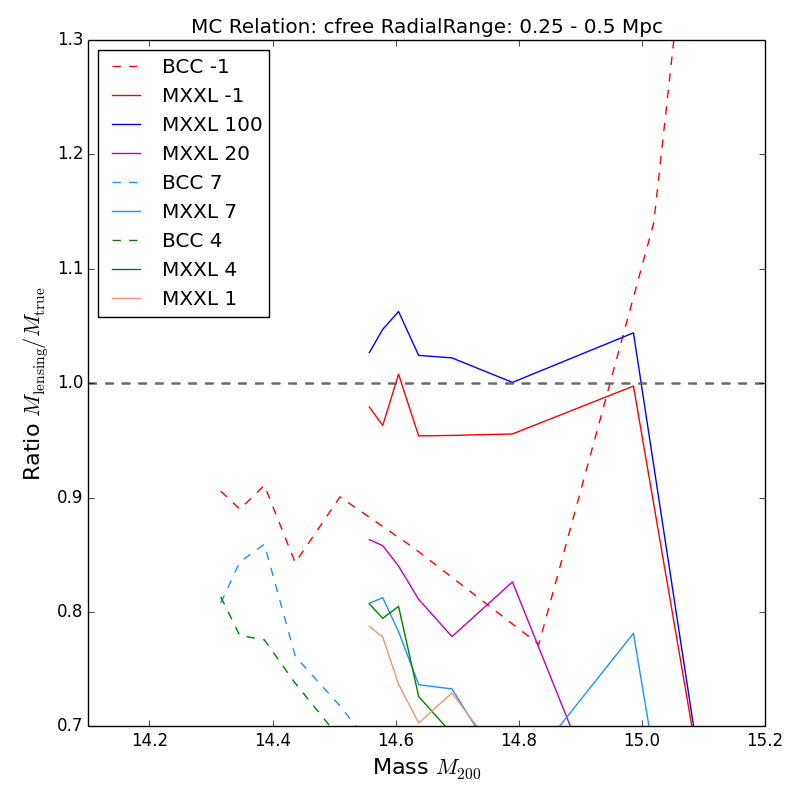
\includegraphics[width=0.3\textwidth]{figures/density_cfree-r1}
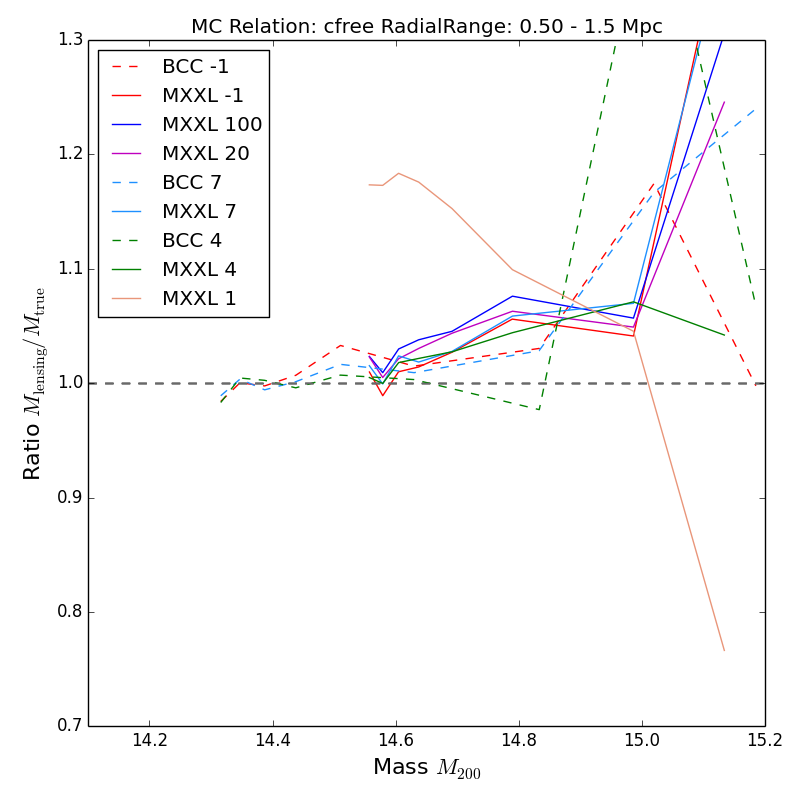
\includegraphics[width=0.3\textwidth]{figures/density_cfree-r5}
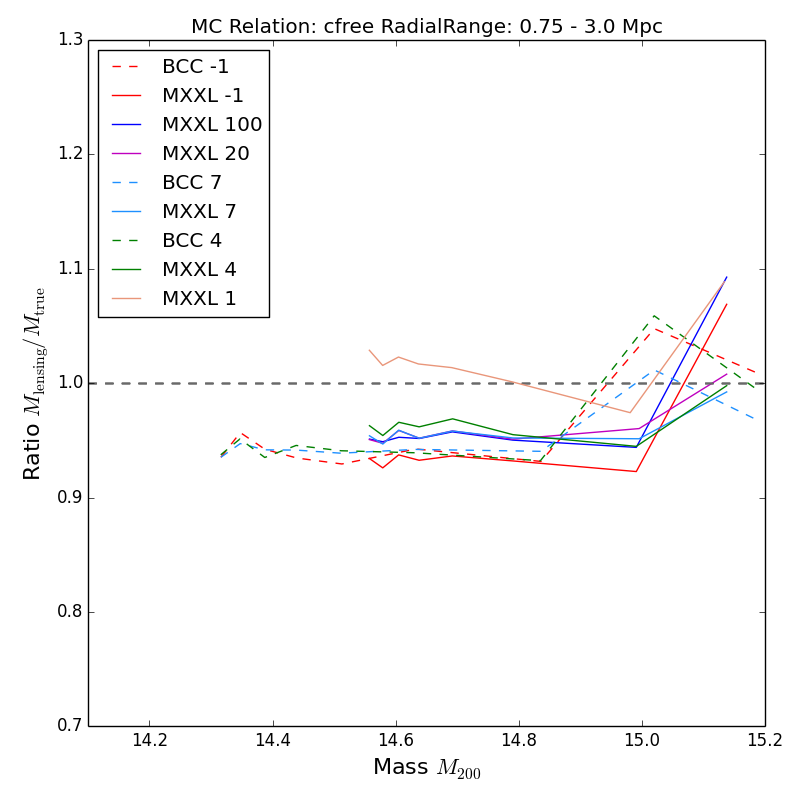
\includegraphics[width=0.3\textwidth]{figures/density_cfree-r10}
\caption{Bias measured from the BCC and MXXL simulations. No shape noise is added, but different sampling densities are used. Left, center, and right are using three different fit radii.}
\label{fig:bcc_vs_mxxl_density}
\end{figure}

We can see the bias comparison in figure~\ref{fig:bcc_vs_mxxl_density}. The center and right panels, fitting and 0.5Mpc and above, show a clean story. I would argue that the simulations roughly agree in the mass range where they have overlapping statistics. The correspondance breaks down a bit in the center panel, but again, rough agreement. In the left panel, we can see that density is really important. With enough sample points, the bias is well behaved (solid red and green curves). But sample sparsely, and the bias jumps up. But the two simulations roughly agree.

\begin{figure} \centering
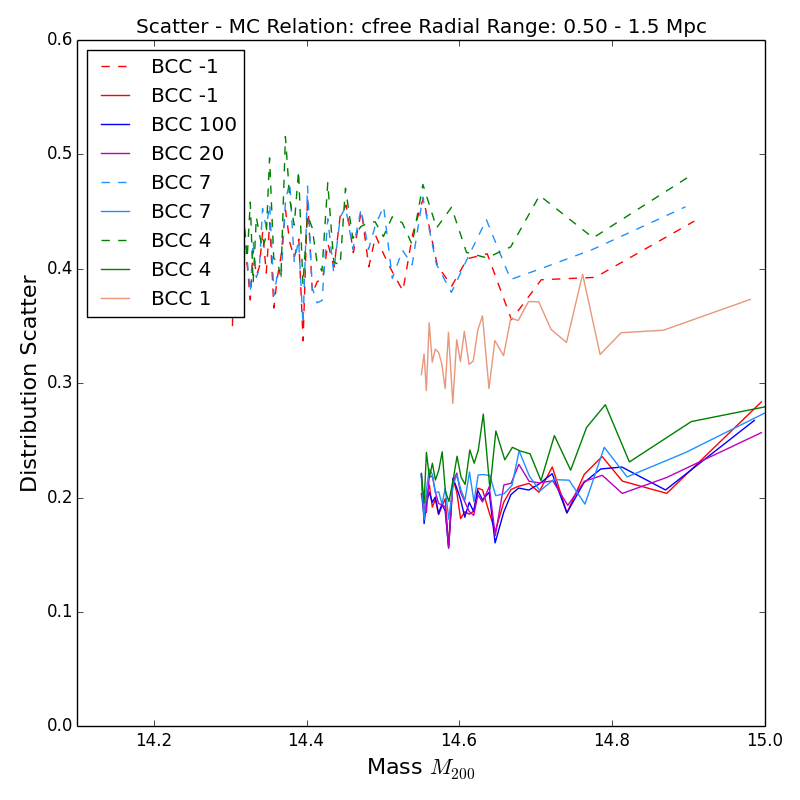
\includegraphics[width=0.4\textwidth]{figures/density_cfree-r5_scatter}
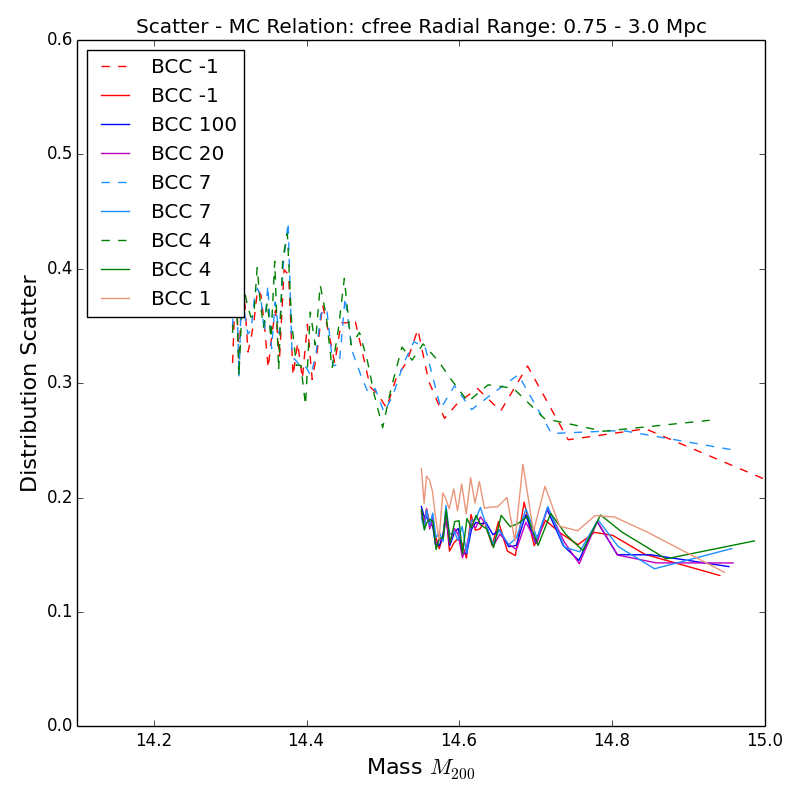
\includegraphics[width=0.4\textwidth]{figures/density_cfree-r10_scatter}
\caption{Comparison of recovered scatters from the two simulations.}
\label{fig:bcc_vs_mxxl_density_scatter}
\end{figure}

When it comes to the scatter, however, the two simulations do not agree. From figure~\ref{fig:bcc_vs_mxxl_density_scatter}, we see that the MXXL has a scatter of ~20\%, practically independent of sampling density. The BCC has a scatter of 30-40\%, with signs of mass dependence. Again, density does not appear to matter. 

\textbf{Why does the scatter not change as the sampling density is reduced (until very low density)?}
10x more noise, when the noise is non-existant, is still non-existant noise, no?

\subsubsection{Is the large scatter in the BCC explained by redshift evolution?}

\textbf{EVIDENCE FOR REDSHIFT-DEPENDENT EVOLUTION!}

I broke down the BCC bias and scatter as a function of mass and redshiftin figure~\ref{fig:bcc_bias_redshift_evo}. This is only for the outer region. However, we see that there does appear to be evolution in the bias and scatter with redshift \emph{and} mass. However, the evolution in bias is < 10\%. I do not think that is enough to explain the extra scatter.

\begin{figure} \centering
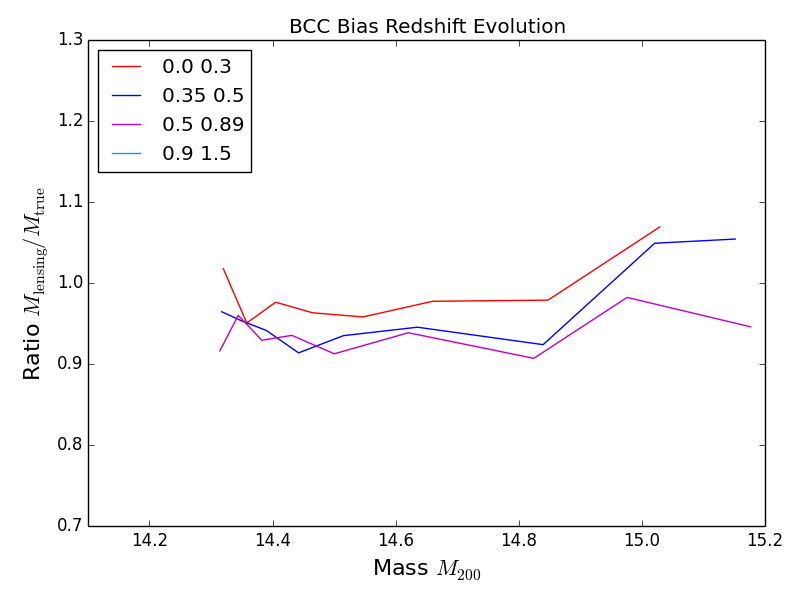
\includegraphics[width=0.8\textwidth]{figures/bcc_bias_redshift_evo_r10_n0_0}
\caption{Evolution of BCC calibration as a function of mass and redshift (colored lines). Left: Bias, Right: Scatter. We do see some redshift evolution(!). It does not appear to be enough to explain the extra scatter in the BCC, but it is important include when trying to calculate the actual bias expected.}
\label{fig:bcc_bias_redshift_evo}
\end{figure}

\textbf{Where is the extra scatter coming from?}

\subsubsection{Sensitivity to Profile Assumptions}

The bias response from assuming an incorrect mass-concentration relation is cosmology dependent \emph{and} radial dependent. In figure~\ref{fig:profile_sensitivity_range_cosmo}, the bias as a function of mass changes with both variables in a way much larger than the difference between different sampling levels.

\begin{figure} \centering
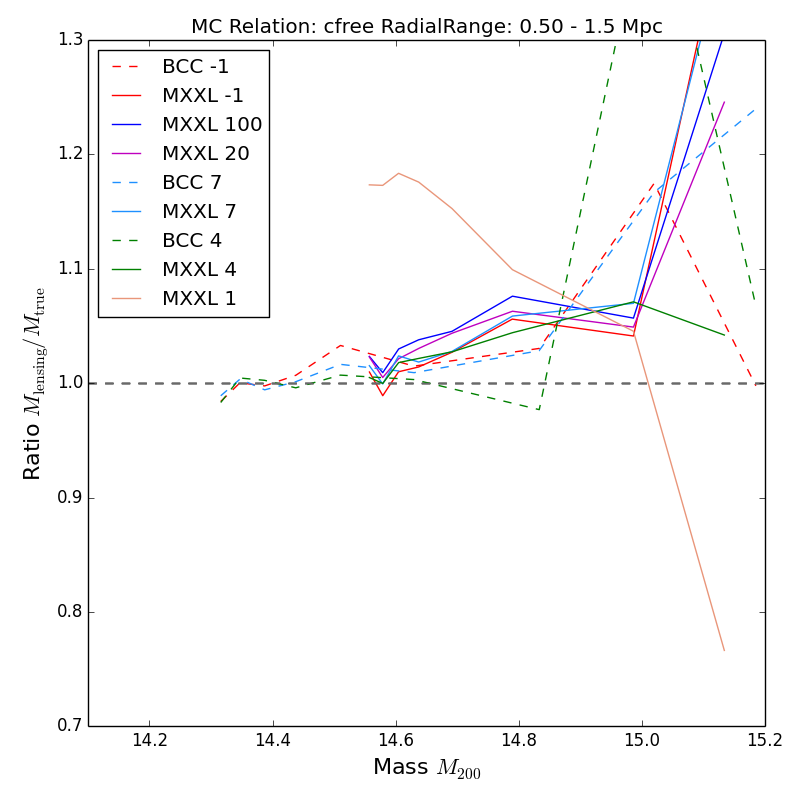
\includegraphics[width=0.4\textwidth]{figures/density_cfree-r5}
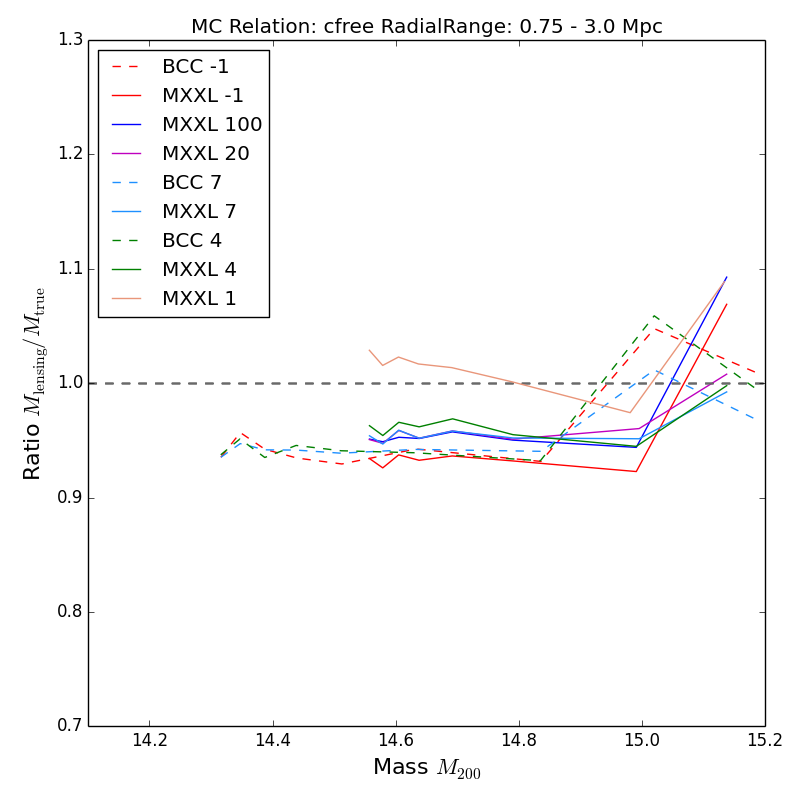
\includegraphics[width=0.4\textwidth]{figures/density_cfree-r10}\\
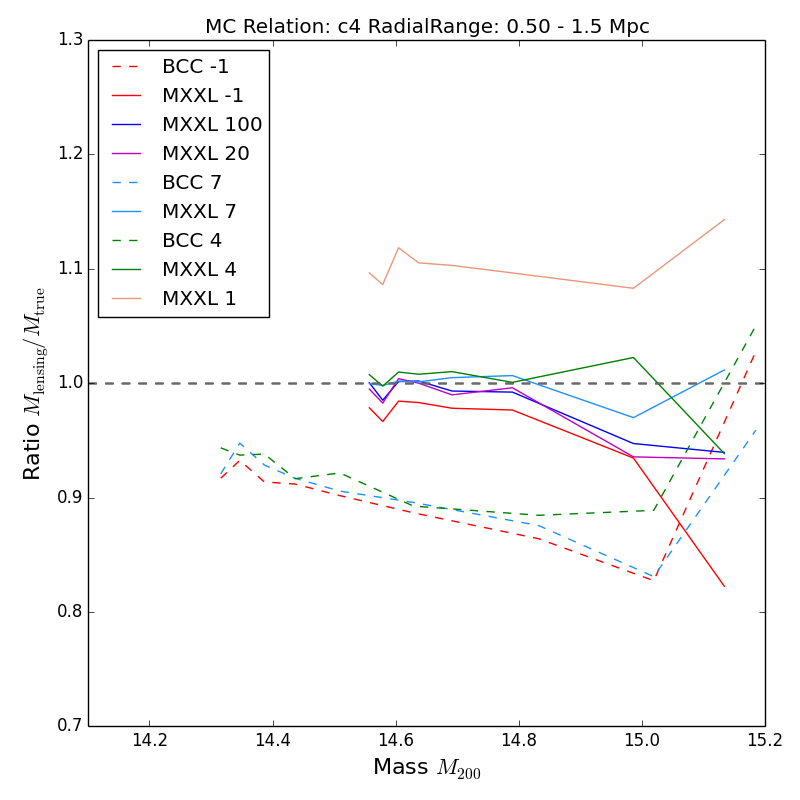
\includegraphics[width=0.4\textwidth]{figures/density_c4-r5}
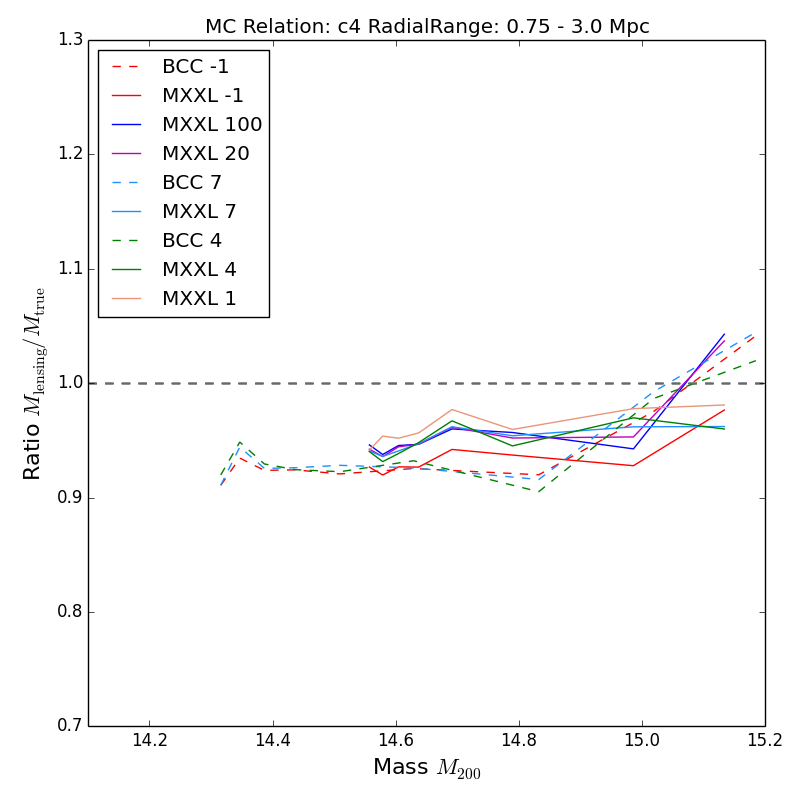
\includegraphics[width=0.4\textwidth]{figures/density_c4-r10}
\caption{A comparison of how the mass-dependent bias changes with cosmology, radial range, mass-concentration relation, and sampling density. Notice how freeing the concentration radically changes the bias, even for high noise simulations.}
\end{figure}

%%%%%%%%%%%%%%%%%%%%%%%%%%%%%%%%%%%%%%%%%%

\subsection{To Consider: If bias depends on cosmology}

I've seen that the two simulations seem to agree when I fit for concentration, at large radii, but that breaks down some at the inner most radii. What if that difference is real, and caused by substructure? What if different cosmologies produce clusters with different amounts of substructure, which lead to different measured biases? 

First, we need to make sure the analysis is robust against substructure and m-c relation. But at some level, \emph{the expected bias has to be cosmology dependent!}

%%%%%%%%%%%%%%%%%%%%%%%%%%%%%%%%%%%%%%%%

\subsection{How does the posterior change as noise is added?}
\label{sec:noisebias_posteriors}

On Monday, I examined how the bias and scatter change as the noise levels change in the simulation. I noticed that the bias tends to increase with increasing noise. I think that is the effect of ``noise bias'', as in the posterior is becoming more skewed at high noise levels. I should be able to see that for individual halos. 

code: inspectProfiles.py
Logfile: logs/noisebias\_probsurface.log

Yeah, this is not working out so well. I think I'll need to table this until later.

%%%%%%%%%%%%%%%%%%%%%%%%%%%%%%%%%%%%%%%

\subsection{How does the bias \& scatter change as noise is added?}
\label{sec:noisebias_bias}

%%%%

\subsubsection{Scatter at high densities}

I'll start with 100 galaxies per sq arcminute. At the outer radii, this is a lot of samples even for noisy galaxies. The behavior of the scatter, however, has some odd radial dependence. See figure~\ref{fig:noisebias_highdensity_radrange}. The smaller fit range has noise that goes up uniformly. That to me suggests the noise is dominated by shape noise. At the outer radii, there are more galaxies included in the fit, so I guess shape noise is suppressed more. OK, not surprising then that the noise rises slower. However, the scatter develops a mass dependence. From the no noise case, we can see that the intrinsic LSS \& triaxial noise is not mass dependent. So maybe this is a signal strength effect, which gets swamped in the shape-noise dominated case at lower radii?

Note that fitting for concentration increases noise, but not radically, except at low radii.

\begin{figure}
\centering
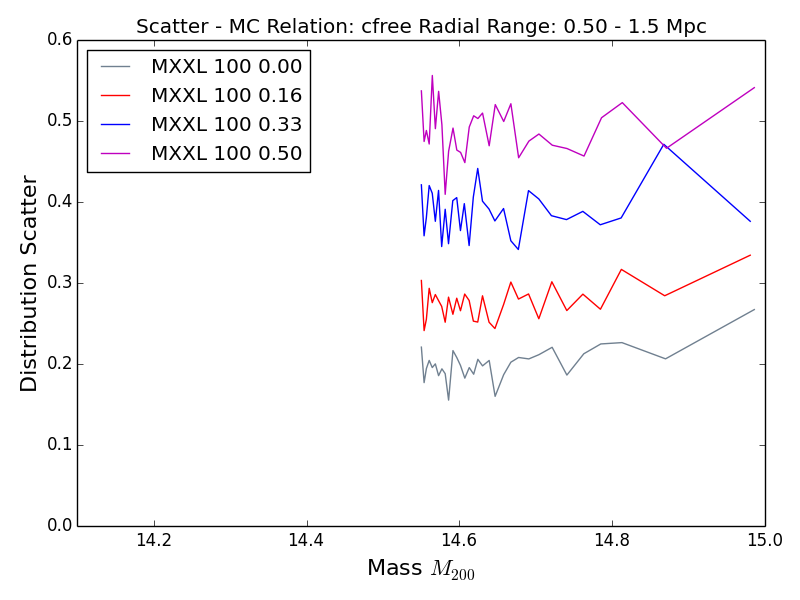
\includegraphics[width=0.4\textwidth]{figures/noise_cfree-r5-n1_3_scatter}
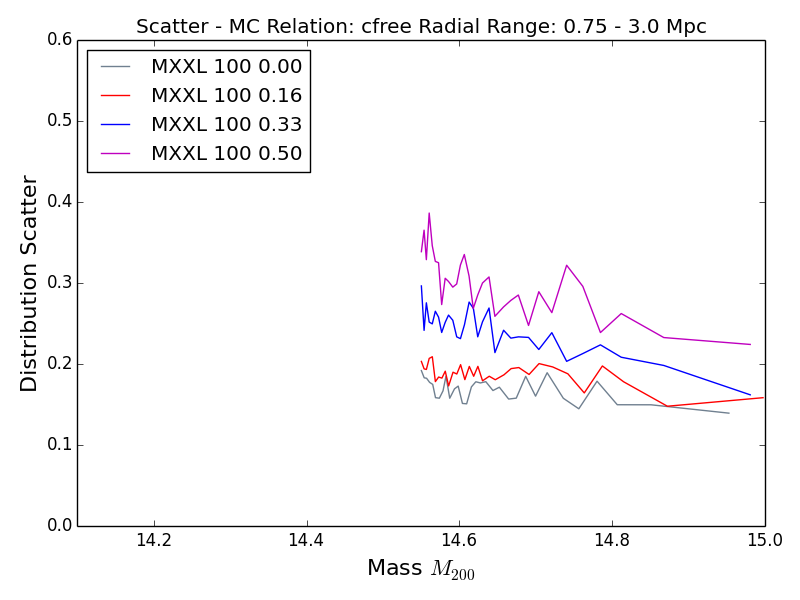
\includegraphics[width=0.4\textwidth]{figures/noise_cfree-r10-n1_3_scatter}\\
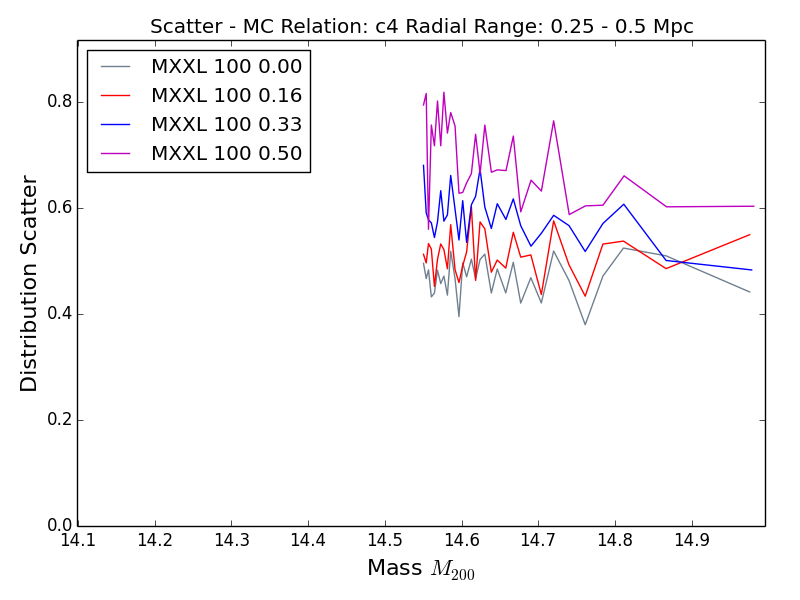
\includegraphics[width=0.4\textwidth]{figures/noise_c4-r5-n1_3_scatter}
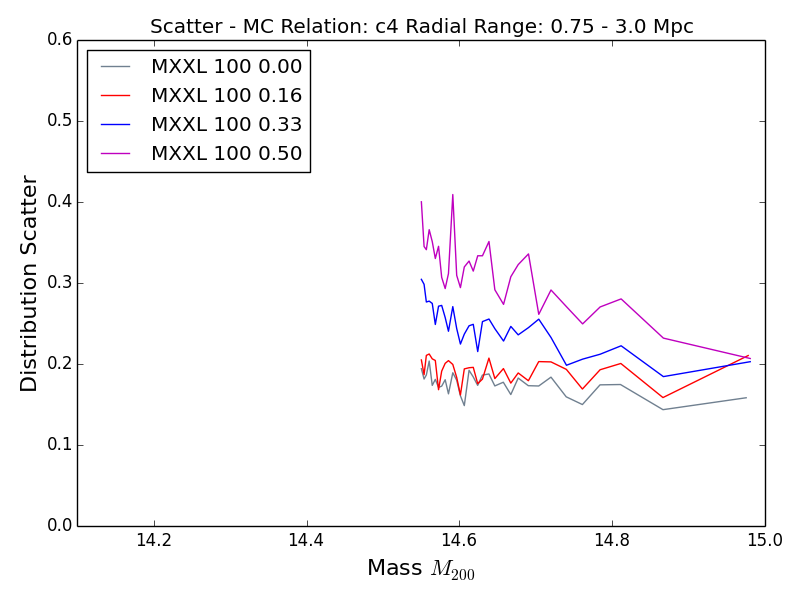
\includegraphics[width=0.4\textwidth]{figures/noise_c4-r10-n1_3_scatter}
\caption{Shown are the measured scatters for 100 galaxies per sq arcminute at different levels of noise. Left column shows fits to 0.5-1.5mpc, whereas the right column shows 0.75 - 3mpc. Top row has concentration free in the fits, the bottom row restricts c=4. Fits to 0.5-1.5mpc behave as I would expect: add shape noise, and the measured scatter goes up. However, fits to 0.75-3mpc show a mass dependence to the noise. While noise goes up, it goes up faster for the low mass galaxies, and at a rate slower than the smaller fit range.}
\label{fig:noisebias_highdensity_radrange}
\end{figure}

%%%%%

\subsubsection{Bias at high densities}

As was seen in \citet{bahe12}, added noise shifts the average bias up. However, at least at 100 galaxies per sq arcmin, the effect is not large, and is somewhat muddled. Also confusing is why the c-free fits to 0.5 - 1.5 mpc develops a mass-dependent bias. See Figure~\ref{fig:noisebias_highdensity_bias}.

\begin{figure}
\centering
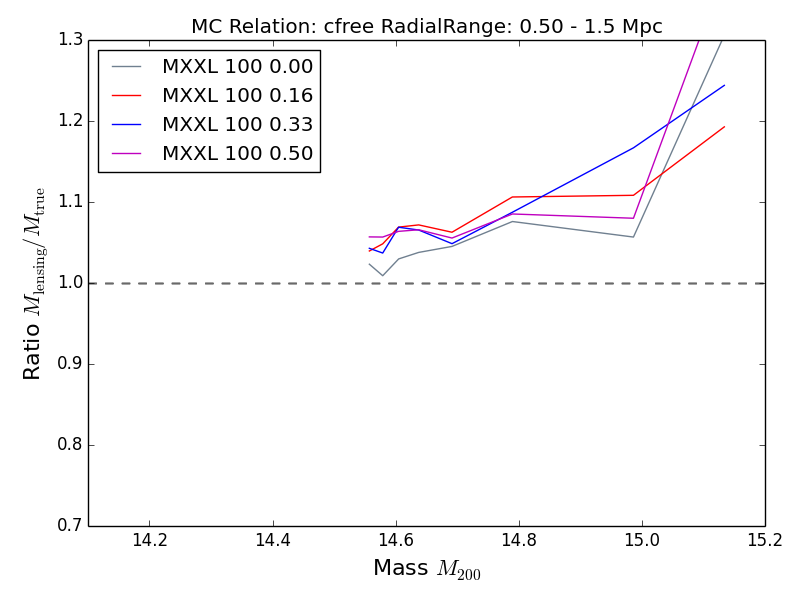
\includegraphics[width=0.4\textwidth]{figures/noise_cfree-r5-n1_3}
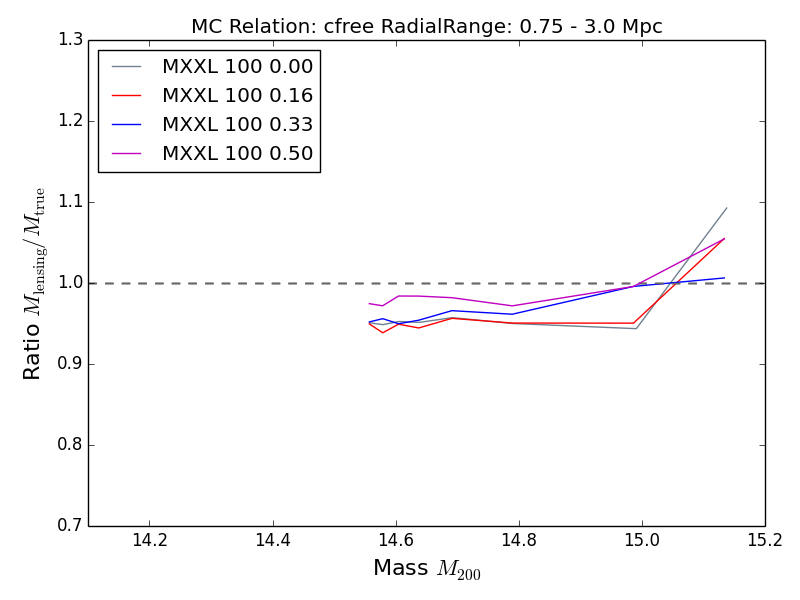
\includegraphics[width=0.4\textwidth]{figures/noise_cfree-r10-n1_3}\\
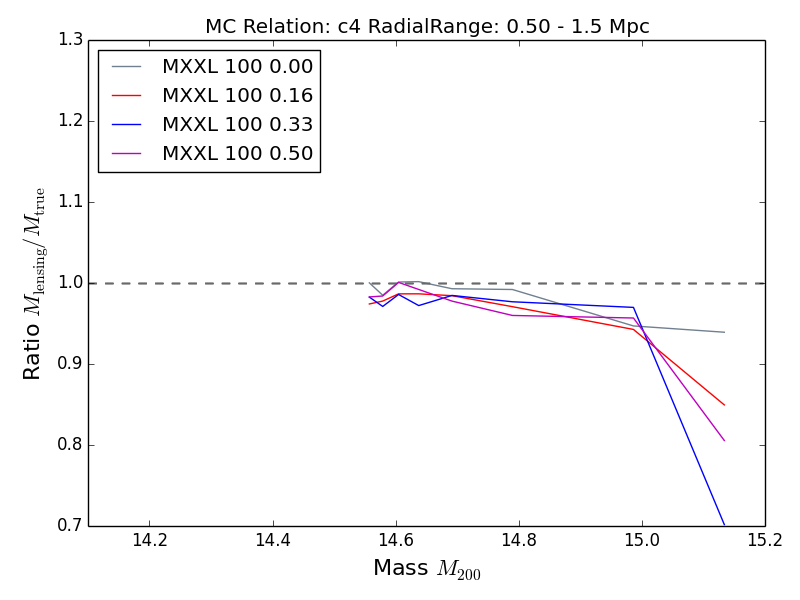
\includegraphics[width=0.4\textwidth]{figures/noise_c4-r5-n1_3}
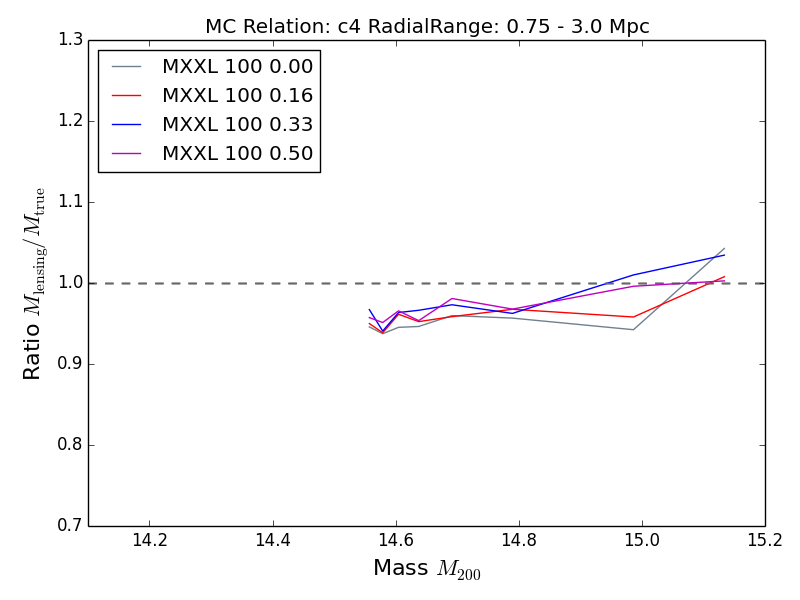
\includegraphics[width=0.4\textwidth]{figures/noise_c4-r10-n1_3}
\caption{Same as fig~\ref{fig:noisebias_highdensity_radrange}, except now I show the bias. What is odd is the c-free fit to 0.5-1.5 mpc, and there is a mass-dependent bias. This was seen previously in multiple figures earlier in this section.}
\label{fig:noisebias_highdensity_bias}
\end{figure}

%%%%%%%

\subsubsection{Bias vs sampling for noisy galaxies}

For the most dramatic example of how noise affects the bias, I turn to noisy galaxies, and change the sampling density at 0.75-3mpc. See figure~\ref{fig:noisebias_noisygals_sparsesampling}.

\begin{figure}
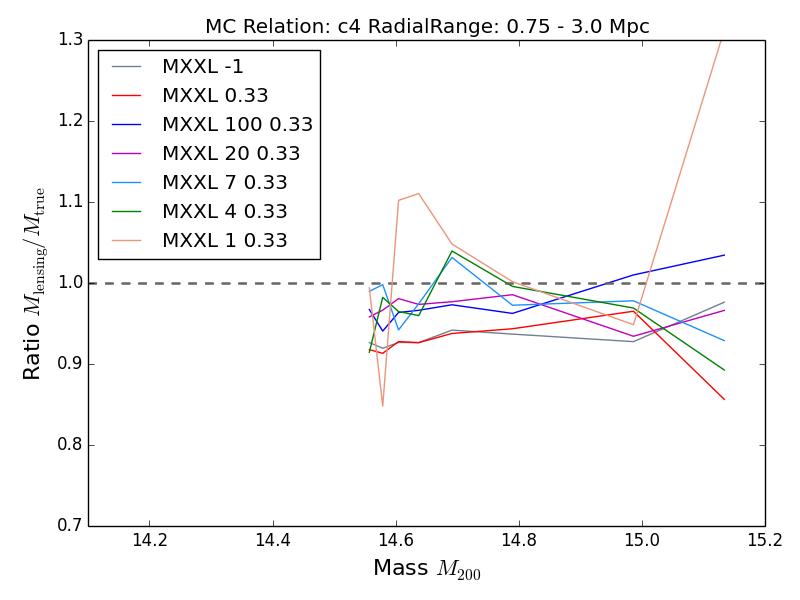
\includegraphics[width=0.4\textwidth]{figures/density_noise2_c4-r10}
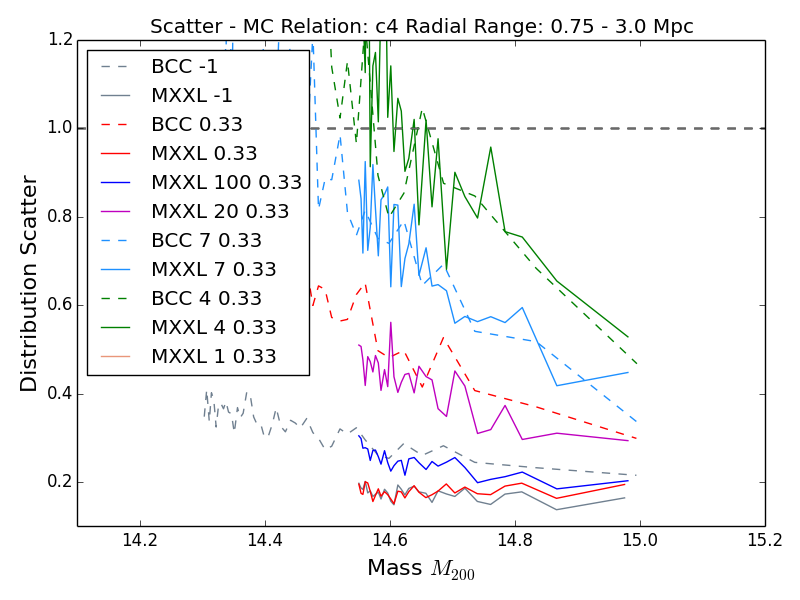
\includegraphics[width=0.4\textwidth]{figures/density_noise2_c4-r10_scatter}\\
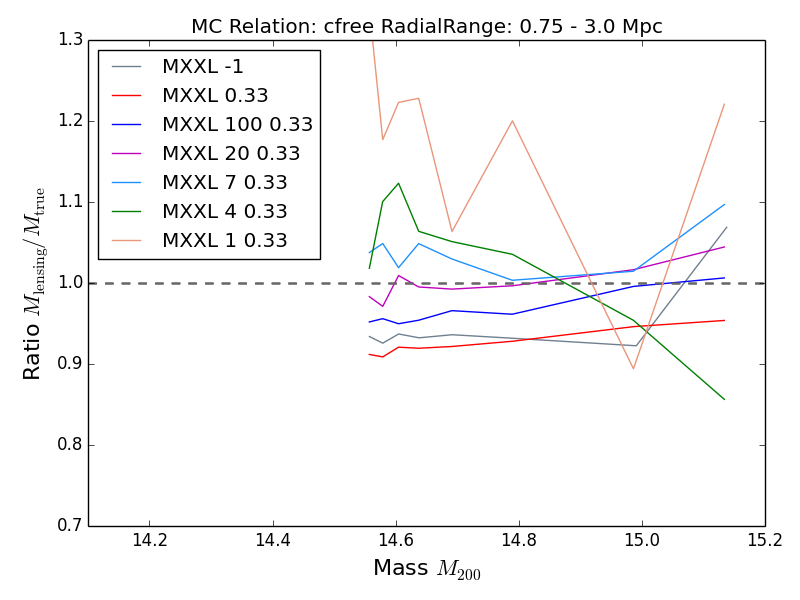
\includegraphics[width=0.4\textwidth]{figures/density_noise2_cfree-r10}
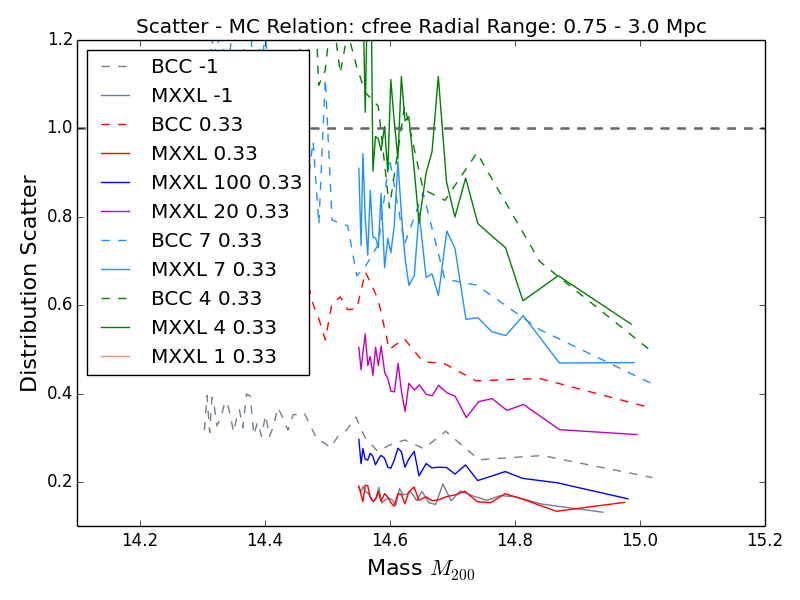
\includegraphics[width=0.4\textwidth]{figures/density_noise2_cfree-r10_scatter}
\caption{Plotted are simulations with increasing noise levels (fit at 0.75-3mpc). Top has c=4, bottom has c-free. The bias is similar at low noise, and seems to shift in similar ways, though the c=4 fit never shifts bias as much as c-free. Interestingly enough, the scatter does not increase dramatically at this radii when concentration is let free. This is in contrast to smaller radii. Obviously fitting for the concentration has an effect, as it changes the bias, but somehow it doesn't change the scatter.}
\end{figure}

Why does bias seems to increase in a mass independent way up to some noise point, after which lower mass clusters develop a steeper bias? The effects aren't as strong with c=4. But I suspect noise bias is at play here. The direction of the bias would suggest skewed posteriors, with tails to to low mass, and high probability density just above the correct mass. I will have to find a way to see that.

%%%%%%%%%%%%%%%

\subsection{Next Steps}

I'd like to create perfect NFW halos, increase noise slowly, and inspect the posterior. That is probably the most clean way to investigate the effects of noise bias. However, what I'm concerned about is that the noise due to LSS \& substructure is not the same as shape noise, where noise is actually correlated between bins. I could imagine that correlated noise could induce difference effects. It would also be nice to model the amount of this correlated noise, so that I could include it in fits. 

%%%%%%%%%%%%%%%%%%%%%%%%%%%%%%%%%%%%%%%%%%%%%%%%%%%%%%%%%%%%%%%%%%%%%%%%%%%%%%%%%%%%%%%%%%%%%%%%%%%%%%%%%%%%%%%%%%%%%%%%%%%%%%%%%%%%%%%%%%%%%%%%%%%%%%%%%%%%%%%%%%%%%%%%%%%%%%%%%%%%%%%%%%%%%%%%%%%%%%%%%%%%
%%%%%%%%%%%%%%%%%%%%%%%%%%%%%%%%%%%%%%%%%%%%%%%%%%%%%%%%%%%%%%%%%%%%%%%%%%%%%%%%%%%%%%%%%%%%%%%%%%%%%%%%%%%%%%%%%%%%%%%%%%%%%%%%%%%%%%%%%%%%%%%%%%%%%%%%%%%%%%%%%%%%%%%%%%%%%%%%%%%%%%%%%%%%%%%%%%%%%%%%%%%%
%%%%%%%%%%%%%%%%%%%%%%%%%%%%%%%%%%%%%%%%%%%%%%%%%%%%%%%%%%%%%%%%%%%%%%%%%%%%%%%%%%%%%%%%%%%%%%%%%%%%%%%%%%%%%%%%%%%%%%%%%%%%%%%%%%%%%%%%%%%%%%%%%%%%%%%%%%%%%%%%%%%%%%%%%%%%%%%%%%%%%%%%%%%%%%%%%%%%%%%%%%%%
\clearpage \newpage

\section{What is the best configuration for the HST Program?}
\label{sec:hstproposal}


\subsection{Motivation}
There are a few different ways we could configure an HST program to observe high-redshift galaxy clusters. We can either take a single-pointing strategy, or some sort of mosaic. There are of course time limitions, and mosaicing will usually mean shallower exposures, with higher shape noise and lower galaxy density. The most effective strategy could also be redshift dependent, as the effective beta and sampling densities change.

\subsection{Setup}
I've used the MXXL to examine this question, by employing different instrument masks. I've introduced a few modifications so that I can approximate what happens when galaxy clusters are at different redshifts. This includes different source densities, different physical distances accepted into the analysis, and different effective betas. Modifications include a new reader class, readMXXL_HSTBeta.py. 

I've used Tim's estimates of Beta, source density, and shape noise from the CANDELS fields. 

From Tim, on 19 Feb. (Note, I clarified that Beta here is D_ls/D_s, not normalized to D_inf.:
\begin{quote}
Hi Doug,

here are my CANDELS estimates for our new HST program with source density, betas and shape noise:


After color cut (V-i<0.4 or V-z<0.45) and S/N cuts (Flux S/N>10):

Source density: (for V-i cut only so far) 

Single pointings: Ngal= 21/arcmin^2 (24<V<26.5) to r=110", probably for z>1 clusters
[3-pt] Mosaics:          Ngal= 16/arcmin^2   (24<V<26)   to r=160"

Shape noise:
0.40 for both components together

Beta:
zl      beta
0.65  0.43  
0.70  0.40  
0.75  0.38   
0.80  0.36       
0.85  0.34   
0.90  0.32   
0.95  0.30   
1.00  0.28
1.05  0.26
1.10  0.24
1.15  0.23
1.20  0.21 
1.25  0.195
1.30  0.18

This is a bit pessimistic given that it uses uniform and not optimal weight, but this can be seen as margin.

Cheers, Tim
\end{quote}

I've set up my code to ``move'' clusters to redshifts 0.7, 0.8, 0.9, 1.0, and 1.1. I've also tested single pointings, 3-pt mosiacs, and 4-pt mosaics based on the existing program. I've assumed the source density for the 4-pointing mosaics to be ~21 galaxies per square arcminute.





%%%%%%%%%%%%%%%%%%%%%%%%%%%%%%%%%%%%%%%%%%%%%%%%%%%%%%%%%%%%%%%%%%%%%%%%%%%%%%%%%%%%%%%%%%%%%%%%%%%%%%%%%%%%%%%%%%%%%%%%%%%%%%%%%%%%%%%%%%%%%%%%%%%%%%%%%%%%%%%%%%%%%%%%%%%%%%%%%%%%%%%%%%%%%%%%%%%%%%%%%%%%
%%%%%%%%%%%%%%%%%%%%%%%%%%%%%%%%%%%%%%%%%%%%%%%%%%%%%%%%%%%%%%%%%%%%%%%%%%%%%%%%%%%%%%%%%%%%%%%%%%%%%%%%%%%%%%%%%%%%%%%%%%%%%%%%%%%%%%%%%%%%%%%%%%%%%%%%%%%%%%%%%%%%%%%%%%%%%%%%%%%%%%%%%%%%%%%%%%%%%%%%%%%%
%%%%%%%%%%%%%%%%%%%%%%%%%%%%%%%%%%%%%%%%%%%%%%%%%%%%%%%%%%%%%%%%%%%%%%%%%%%%%%%%%%%%%%%%%%%%%%%%%%%%%%%%%%%%%%%%%%%%%%%%%%%%%%%%%%%%%%%%%%%%%%%%%%%%%%%%%%%%%%%%%%%%%%%%%%%%%%%%%%%%%%%%%%%%%%%%%%%%%%%%%%%%
\clearpage \newpage

\section{What is the best mass to measure?}

The above work was done looking at M200. However, as it currently stands, we are calibrating masses closer to M500. There is also an open question as to what mass is the least sensitive to m-c assumptions, or put another way, what is the mass that lensing measures the best?

To start, I'd like to remake the above plots with M500 instead of M200. However:

\begin{itemize}
\item The BCC M500 values appear to be larger than the M200 values
\item The MXXL M500 values that I have are for the z=0 slice, not the z=1 slice.
\end{itemize}

I've contacted Aaron about the MXXL problem, but I am holding off contacing Matt about the BCC issue until I am ready to show him some preliminary results.



%%%%%%%%%%%%%%%%%%%%%%%%%%%%%%%%%%%%%%%%%%%%%%%%%%%%%%%%%%%%%%%%%%%%%%%%%%%%%%%%%%%%%%%%%%%%%%%%%%%%%%%%%%%%%%%%%%%%%%%%%%%%%%%%%%%%%%%%%%%%%%%%%%%%%%%%%%%%%%%%%%%%%%%%%%%%%%%%%%%%%%%%%%%%%%%%%%%%%%%%%%%%
%%%%%%%%%%%%%%%%%%%%%%%%%%%%%%%%%%%%%%%%%%%%%%%%%%%%%%%%%%%%%%%%%%%%%%%%%%%%%%%%%%%%%%%%%%%%%%%%%%%%%%%%%%%%%%%%%%%%%%%%%%%%%%%%%%%%%%%%%%%%%%%%%%%%%%%%%%%%%%%%%%%%%%%%%%%%%%%%%%%%%%%%%%%%%%%%%%%%%%%%%%%%
%%%%%%%%%%%%%%%%%%%%%%%%%%%%%%%%%%%%%%%%%%%%%%%%%%%%%%%%%%%%%%%%%%%%%%%%%%%%%%%%%%%%%%%%%%%%%%%%%%%%%%%%%%%%%%%%%%%%%%%%%%%%%%%%%%%%%%%%%%%%%%%%%%%%%%%%%%%%%%%%%%%%%%%%%%%%%%%%%%%%%%%%%%%%%%%%%%%%%%%%%%%%
\clearpage \newpage

\section{Collaborators, Acknowledgements, Debts}

\subsection{Collaborators}

Stanford
\begin{itemize}
\item Steve Allen
\item Anja von der Linden
\item Pat Kelly
\item Adam Mantz
\item Glenn Morris
\end{itemize}

Bonn
\begin{itemize}
\item Tim Schrabback
\item Peter Schneider
\end{itemize}

SPT
\begin{itemize}
\item Brad Benson
\item Joerg Dietrich
\end{itemize}

MXXL Simulations
\begin{itemize}
\item Stefan Hilbert
\end{itemize}

BCC Simulations
\begin{itemize}
\item Risa Wechsler
\item Matt Becker
\item Michael Buscha
\end{itemize}

BK11 Simulations
\begin{itemize}
\item Matt Becker
\end{itemize}


%%%%%%%%%%%%%%%%%%%%%%%%%%%%

\bibliography{refs.bib}

%%%%%%%%%%%%%%%%%%%%%%%%%%%%%



\end{document}

